% arara: xelatex: { shell : yes }
% arara: biber
% arara: xelatex: { shell : yes }
% arara: xelatex: { shell : yes }

% options:
% thesis=B bachelor's thesis
% thesis=M master's thesis
% czech thesis in Czech language
% slovak thesis in Slovak language
% english thesis in English language
% hidelinks remove colour boxes around hyperlinks

\documentclass[thesis=B,czech]{template/FITthesis}[2019/12/23]

% \usepackage{amsmath} %advanced maths
% \usepackage{amssymb} %additional math symbols

\usepackage{dirtree} %directory tree visualisation
\usepackage{polyglossia}
\setmainlanguage{czech}
\usepackage{graphicx}
\usepackage{url}
\usepackage{hyperref} % [hidelinks]
\usepackage{csquotes} % dává české enquotes
\usepackage{xevlna}

\usepackage{minted}
\counterwithin{listing}{chapter}
\renewcommand{\listingscaption}{Výpis kódu}
\renewcommand{\listoflistingscaption}{Seznam výpisů kódu}

\usepackage[style=iso-numeric,backend=biber]{biblatex}
\addbibresource{bibliography.bib}

% % list of acronyms
% \usepackage[acronym,nonumberlist,toc,numberedsection=autolabel]{glossaries}
% \iflanguage{czech}{\renewcommand*{\acronymname}{Seznam pou{\v z}it{\' y}ch zkratek}}{}
% \makeglossaries


% % % % % % % % % % % % % % % % % % % % % % % % % % % % % % 
% ODTUD DAL VSE ZMENTE
% % % % % % % % % % % % % % % % % % % % % % % % % % % % % % 

\department{Katedra softwarového inženýrství}
\title{Automatický provisioning herních serverů pomocí cloudové image}
\authorGN{Matyáš} %(křestní) jméno (jména) autora
\authorFN{Ješina} %příjmení autora
\authorWithDegrees{Matyáš Ješina} %jméno autora včetně současných akademických titulů
\author{Matyáš Ješina} %jméno autora bez akademických titulů
\supervisor{Ing. Tomáš Vondra, Ph.D.}
\acknowledgements{Doplňte, máte-li komu a za co děkovat. V~opačném případě úplně odstraňte tento příkaz.}
\abstractCS{Tato práce se zabývá problematikou automatického nasazování herních serverů a jejich provozu v cloudovém prostředí.
Zkoumá možnosti nasazování aplikací v cloudu za účelem nalezení nejefektivnějšího způsobu
a popisuje vytvoření obrazu systému, který je pro dané využití vhodný. Tento systém je schopný podporovat množství herních serverů
bez nutnosti jeho časté změny a je snadno rozšiřitelný i pro další hry v budoucnosti.

Výsledkem je obraz systému určeného pro provoz herních serverů, který je bezpečný, obsahuje jen nezbytně nutné součásti a dá se jednoduše nasadit v cloudovém prostředí.
Celý proces jeho sestavení je plně automatizovaný.}
\abstractEN{This thesis addresses the possibilities of automatic deployment and provisioning of game
servers in cloud environment. It explores existing possibilities of deploying applications in cloud to find the optimal solution
and describe the creation of a system image appropriate for this use case. This system is capable of running various game servers without frequent
changes to its internal structure and is easily modifiable to include more games, if desired.

The result si a system image designated to run game servers, which is secure,
contains only the most necessary components, and can easily be deployed to cloud environment. The entire
process is fully automated.}
\placeForDeclarationOfAuthenticity{V~Praze}
\declarationOfAuthenticityOption{4} %volba Prohlášení (číslo 1-6)
\keywordsCS{herní server, počítačová hra, cloud, automatizace, nasazování systému}
\keywordsEN{game server, video game, cloud, automatization, system deployment}
% \website{http://site.example/thesis} %volitelná URL práce, objeví se v tiráži - úplně odstraňte, nemáte-li URL práce

\begin{document}

\begin{introduction}

Počítačové hry se těší velké popularitě. S rozšířením internetu začaly vznikat také hry
pro více hráčů, které se rychle dostaly do čela žebříčků oblíbenosti a dnes jsou zábavou pro stovky milionů
hráčů po celém světě.

Mnohé z těchto her umožňují uživatelům vytvořit vlastní herní servery, na kterých je možné hrát s přáteli
či jinou komunitou.
Pokud chce uživatel zprovoznit herní server, měl by takový postup být jednoduchý a rychlý.
Je možné provozovat server na vlastním počítači, zde je však kvalita herního zážitku 
ovlivněna konfigurací systému a internetovým připojením. Také je často potřeba pokročilého nastavení
směrovače, který herní server z domácí sítě zpřístupní do internetu.

Tato práce se zaměřuje na další možnost provozu těchto serverů, a to v cloudovém prostředí. Uživatel se tak nemusí zabývat 
kvalitou internetového připojení či manuálním nastavováním síťových prvků. Herní servery
pro menší počet hráčů jsou často vytvářeny a rušeny, nasazení v cloudu tedy představuje ideální způsob provozu,
kde jsou tyto operace jednoduché a automatizovatelné.

Cílem práce je vytvořit obraz systému, který bude pro toto použití vhodný. Uživatel bude mít možnost vybrat
požadovaný herní server a systém provede všechny operace potřebné k jeho zprovoznění.

Výsledek práce bude prospěšný zejména pro stávající uživatele cloudových služeb, kteří mají alespoň minimální
zkušenosti s nasazováním obrazů systémů. S minimální interakcí budou mít možnost spustit herní server dle svého
výběru bez složité instalace a konfigurace. Pokročilí uživatelé využijí možnosti automatizace celého procesu,
která jim zaručí rychlé spuštění vybraného serveru za pomoci několika příkazů.

Vytvořený obraz musí být snadno dostupný a zdokumentovaný, jednoduchý na nasazení, s minimální náročností 
na systémové prostředky. Bude jej také možné využít v komerčním prostředí.

\end{introduction}
\chapter{Cíl práce}

Hlavním cílem této práce je vytvořit obraz systému, který bude schopný provozovat herní servery v cloudovém prostředí.
Tento systém musí být jednoduchý na zprovoznění i úpravy. Bude tedy ideálním kandidátem pro uživatele se základní znalostí
nasazování serverů v cloudu, který nechce provozovat herní server na vlastní infrastruktuře.
Práce se zaměří na herní servery pro menší množství hráčů (přibližně do 50), které obecně vyžadují méně systémových prostředků a nastavení
a proces jejich vytváření je tak jednoduše automatizovatelný.

V první části práce je tedy nutné analyzovat dostupné možnosti a najít výhody a nevýhody daných řešení. Dále je potřeba vybrat
vhodný operační systém, který splňuje dané požadavky. V dalším kroku budou porovnány různé možnosti provozu herních serverů
na daném systému a jejich automatizace.

V praktické části bude implementována součást pro interaktivní i automatickou instalaci herních serverů a jejich provoz. Jelikož je kladen důraz
na jednoduchost provozu, musí tento program pracovat s uživatelsky přívětivým prostředím, případně plně automaticky.
Tato součást také musí být schopna spouštět a zastavovat herní server, bude-li to nutné.

Jelikož se bude po nasazení jednat o veřejně dostupný systém, je zde důležitým prvkem jeho bezpečnost. Budou tedy vyhodnoceny možnosti
jeho zabezpečení, zahrnující například vzdálený přístup.
\chapter[Současná řešení]{Současná řešení}

V této části budou prozkoumána existující řešení pro vytváření herních serverů.
Vzhledem k velkému množství herních serverů existuje také mnoho způsobu jejich provozu a údržby. Aplikace nabízené přes platformu Steam
lze například spravovat pomocí nástroje SteamCMD \cite{steamcmd}, avšak tento způsob neumožňuje provozovat herní servery jiných společností.
Z tohoto důvodu existují aplikace na správu herních serverů, které umožňují spouštět servery od mnoha společností uživatelsky přívětivou cestou.
Tyto aplikace jsou zpravidla provozovány v samostatném operačním systému, aby byl zajištěn plynulý chod.
Mnohé z nich podporují systém plateb za provoz herních serverů a jsou tak vhodné pro komerční využití.

\section{GameCP}

Jedním z pokročilých nástrojů pro správu herních serverů je Game Control Panel \cite{gamecp}. Jedná se o administrátorský nástroj pro společnosti
zabývající se pronájmem herních serverů. Tato aplikace umožňuje uživatelům spravovat velké množství herních serverů pomocí webového klienta,
který je přehledný a snadno přizpůsobitelný. Aplikace podporuje možnost evidence plateb za herní servery a poskytuje prostředí pro poskytování
podpory klientům, kteří si herní servery pronajímají. Kromě herních serverů podporuje nástroj také práci s programy pro komunikaci, jako jsou TeamSpeak
nebo Ventrilo. Jedná se o placenou aplikaci s měsíčním předplatným bez dostupného zdrojového kódu.

\section{Pterodactyl}

Pterodactyl \cite{pterodactyl} je dalším z nástrojů pro správu herních serverů, který poskytuje přehledné webové rozhraní pro vytváření herních serverů.
Podporuje množství herních serverů a umožňuje uživatelům vytvářet instance serverů pomocí Docker kontejnerů. Jedná se o bezplatný nástroj
s volně dostupným zdrojovým kódem, který podporuje provoz množství herních serverů na jednom zařízení. Tento systém je aktivně vyvíjen komunitou
a zakládá si na jednoduchosti a kvalitní dokumentaci. API umožňuje komplexní přístup k jednotlivým funkcím a nabízí tak možnost automatizace
vytváření serverů.

\section{GameserverApp}

Dalším z existujících placených nástrojů je GameserverApp \cite{gameserverapp}. Jedná se o systém zaměřený na propojení komunikační platformy Discord s herními servery.
Umožňuje zpoplatnění herních funkcí a poskytování speciálních funkcí na plaftormě Discord platícím hráčům. Podporuje automatizované vytváření herních serverů, nabízí však jen
minimální množství her. Pro uživatele bez vlastního serveru poskytuje také pronájem vlastních serverů. Nástroj je zpoplatněný s neveřejným zdrojovým kódem.

% Mezi existující nástroje se řadí například:
% \begin{itemize}
%     \item GameCP -- placený nástroj pro správu herních serverů,
%     \item Pterodactyl -- aplikace pro správu mnoha herních serverů na různých systémech,
%     \item PufferPanel -- podobná aplikace jako Pterodactyl, s menším množstvím podporovaných her,
%     \item LinuxGSM -- sada skriptů pro správu herních serverů,
%     \item Open Game Panel -- správce herních serverů, nyní již neudržovaný.
% \end{itemize}
% Mnohé z těchto aplikací jsou vhodné pro správu velkého množství herních serverů, které běží na různých systémech. Díky webovému rozhraní umožňují snadný
% přístup pro administrátory, případně i zavedení platebního systému pro zákazníky. Jsou tedy vhodné převážně pro komerční subjekty, které se zabývají
% provozem herních serverů pro zákazníky. Většina jejich funkcí je pro tuto práci zbytečná.
\chapter{Rešerše technologií}

V této kapitole je popsán výběr technologií vhodných pro tvorbu požadovaného systému.
Vzhledem k množství existujících her a četnosti jejich aktualizací není vhodné vytvářet vlastní
systém pro jejich správu, bude tedy nezbytné využít již existujících správců herních serverů.

\section{Operační systém}

Tato sekce uvede možné operační systémy pro provoz herních serverů v cloudovém prostředí a zhodnotí
jejich výhody a nevýhody. Budou zde zhodnoceny pouze obecně rozšířené serverové operační systémy \cite{server_os_share} a jejich deriváty,
aby byla zajištěna podpora a maximální možná bezpečnost.

\subsection{Windows Server}

Jeden z nejrozšířenějších operačních systémů pro serverové využití. Jedná se o komplexní systém s relativně velkými požadavky na
systémové prostředky, který je vhodný i pro rozsáhlé aplikace. Pravidelné aktualizace zajišťují bezpečnost, k dispozici je technická
podpora pro zákazníky. Windows Server je systém s uzavřeným zdrojovým kódem a pro jeho provozování je nutné zakoupit licenci,
není tedy vhodný pro spuštění jednoduchého herního serveru.

\subsection{Linux}



\section{Správce herních serverů}
Nástroj LinuxGSM je zaměřen na jednoduchou instalaci a správu herních serverů pomocí skriptů z prostředí příkazové řádky \cite{linuxgsm}. 
\chapter[Analýza a návrh]{Analýza a návrh}

\section{Požadavky}

Vzhledem k rostoucí popularitě cloudových služeb \cite{statista_cloud_revenue} existuje množství zdrojů, ze kterých lze čerpat.
Herní servery se oproti ostatním typům běžných cloudových aplikací odlišují svojí vysokou náročností
na systémové prostředky, mimo jiné například požadavkem na nízkou latenci.

Při provozování cloudového serveru pro velké množství hráčů je nutné zajistit správné fungování infrastruktury,
jako je například správné vyvažování zátěže mezi jednotlivé servery či automatický výběr nejvhodnějšího serveru
pro klienta \cite{building_cloud_mog_server}. Tyto problémy zde není nutné řešit -- výsledek práce má sloužit jako jednoduchý a rychlý
způsob nasazení herního serveru, není tedy z principu vhodný pro dlouhodobé obsluhování velkého množství hráčů.

U poskytovatelů cloudových serverů je možné vybrat množství systémových prostředků, které bude mít aplikace k dispozici.
Pokud sledujeme vytížení herních serverů v čase, můžeme spatřit jisté vzory, například nárůst hráčů ve večerních hodinách.
Jedná-li se o velký rozdíl v množství uživatelů, je nutné dynamicky navyšovat systémové prostředky \cite{efficient_resources}.
Stejně jako dříve zmíněný problém se i tento týká převážně aplikací pro velké množství uživatelů, v rámci této práce tedy tento problém není uvažován.
Již přidělené prostředky nemůže vytvořený systém nijak ovlivnit, jejich výběr bude tedy ponechán na uživateli před spuštěním.

Důležitým prvkem kteréhokoliv systému je zabezpečení. Aplikace musí být s důrazem na bezpečnost nejen provozována,
ale i vytvářena \cite{newcombe_2012}. Bezpečnostní nedostatek může pro potenciálního útočníka znamenat možnost neoprávněného vstupu do systému.
Budou tedy prozkoumána dostupná bezpečností řešení pro cloudové aplikace.

Obraz systému musí být schopný nainstalovat a spustit herní server automaticky, případně pouze s nezbytně nutnou interakcí uživatele.
Bude proveden průzkum dostupných možností pro automatickou instalaci herních serverů za účelem výběru vhodného řešení.
Spouštění i zastavování herních serverů musí být plně automatizovatelné.

\section{Operační systém}

\section{Správce herních serverů}
\chapter{Implementace}

Tato kapitola popisuje proces implementace navrhnutého řešení a popisuje použité nástroje.
Systém byl implementován podle návrhu v předchozí kapitole.
Dále jsou zde obsaženy vybrané ukázky kódu a výsledné podoby systému.

\section{Nástroje}

\subsection{Editor}

Pro vývoj kódu byl použit editor Visual Studio Code \cite{vscode}, který umožňuje snadnou integraci s verzovacím systémem
a podporuje množství typů souborů. Pomocí rozšiřujících doplňků je možné doplnit editor o pokročilé funkce či podporuj
dalších programovacích jazyků.

\subsection{Verzování}

K verzování projektu byl využit verzovací nástroj Git \cite{git}. Tento volně dostupný nástroj nabízí
neomezené distribuované verzování a je vhodný pro správu kódu.
Kód byl pomocí nástroje ukládán na webový server GitHub, který využívají i používané systémy TurnKey GNU/Linux
a LinuxGSM.

\subsection{Prostředí pro tvorbu obrazu}

Pro sestavení obrazu byl využit operační systém TKLDev \cite{tkldev}, provozovaný jako lokální virtuální stroj. Tento systém, spravovaný vývojáři TurnKey GNU/Linux,
je určen pro tvorbu nových obrazů této distribuce s přednastavenou aplikací. Umožňuje vytvářet obrazy ve formátech pro virtuální stroje a podporuje
také tvorbu obrazů určených k provozu u poskytovatelů cloudových služeb.

\section{Ukázky}

\subsection{Interaktivní výběr herního serveru}

Na obrázku \ref{fig:game-selection} je zobrazen interaktivní výběr herního serveru. Tento výběr je automaticky
k dispozici při prvním spuštění systému, pokud uživatel neurčil herní server pomocí inicializačního skriptu.

\begin{figure}[h]
    \centering
    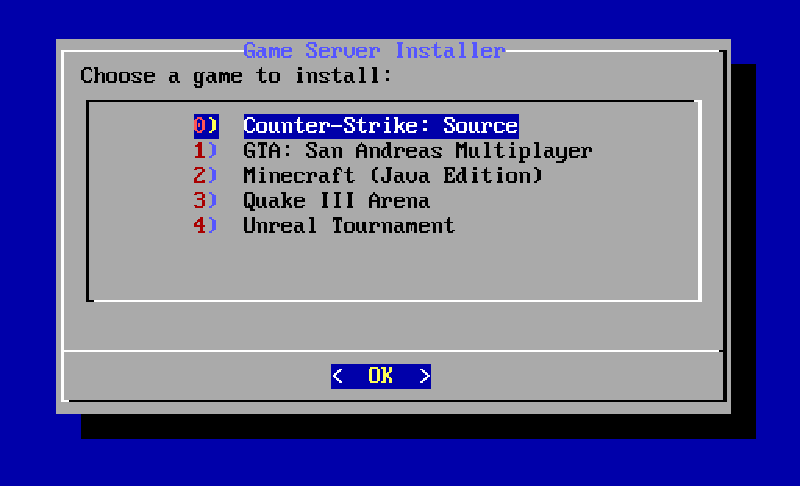
\includegraphics[width=1\linewidth]{chapters/images/game-selection.pdf}
    \caption{Interaktivní výběr hry při prvním spuštění}
    \label{fig:game-selection}
\end{figure}

\subsection{Automatický výběr herního serveru}

V případě plně automatického nasazení herního serveru je nutné použít inicializační skript, který před prvním spuštěním systému
zapíše do souboru \mintinline{shell}{/etc/inithooks.conf} potřebná data pro automatickou konfiguraci systému.
V ukázce \ref{code:init-script} je uveden inicializační skript, pomocí kterého dojde k instalaci herního serveru pro hru \mintinline{shell}{GTA: San Andreas Multiplayer}
včetně nastavení administrátora serveru.

\newpage

\begin{listing}[h!]
    \caption{Ukázkový inicializační skript}
    \label{code:init-script}
    \begin{minted}{shell}
#!/bin/bash

cat>/etc/inithooks.conf<<EOF
export ROOT_PASS=SecretRootPassword
export DB_PASS=SecretMysqlPassword
export APP_PASS=SecretGameuserPassword
export APP_EMAIL=admin@example.com
export HUB_APIKEY=SKIP
export SEC_UPDATES=FORCE

export GAME=samp
export GAME_RCON_PASS=GameserverAdminPassword
EOF
    \end{minted}
\end{listing}

\subsection{Přidání nové hry}

Ukázky \ref{code:game-props-script} a \ref{code:game-config-script} demonstrují přidání podpory pro nový herní server. Jedná se o dva skripty správce herních serverů,
které zavádějí podporu pro server hry \mintinline{shell}{Minecraft} a umožňují jeho minimální počáteční konfiguraci.
Skript \mintinline{shell}{game_properties.sh} zavádí proměnné, které jsou instalačním programem využity k identifikaci herního serveru.
Druhý skript poté umožňuje nastavit uživatelské jméno administrátora serveru pomocí předdefinované proměnné, případně interaktivně.

\begin{listing}[h]
    \caption{Skript \mintinline{shell}{game_properties.sh}}
    \label{code:game-props-script}
    \begin{minted}{shell}
GAME="mc"
GAME_LONG_NAME="Minecraft (Java Edition)"
    \end{minted}
\end{listing}

\begin{listing}[h]
    \caption{Skript \mintinline{shell}{post_install.sh}}
    \label{code:game-config-script}
    \begin{minted}{shell}
#!/bin/bash

# Set server admin
if [ -z "$GAME_ADMIN" ]; then
    read -p "Server admin username: " GAME_ADMIN || GAME_ADMIN=''
    echo
fi
run_as_user "echo \"$GAME_ADMIN\" > \"$GAMEDIR/serverfiles/ops.txt\""
    \end{minted}
\end{listing}

\section{Možnosti rozšíření}

Systém v současné době podporuje pouze čtyři herní tituly. Díky decentralizovanému návrhu
a osamostatnění části pro správu herních serverů od operačního systému je však možné doplňovat podporu
pro další herní servery bez zásahu do obrazu systému.

Některé herní servery vyžadují před spuštěním přihlášení k platformě Steam za účelem ověření zakoupení licence
pro jejich provoz. Tyto servery nejsou v současné chvíli systémem podporovány. V případě jejich podpory
by bylo nutné získat od uživatele jeho přihlašovací údaje, pomocí kterých by bylo možné licenci ověřit.

Systém je díky možnosti plně automatického spuštění vhodný i pro provoz v komerčním prostředí, vzhledem k aktuálnímu
množství podporovaných her ale není konkurenceschopný.


\chapter{Testování}

Tato kapitola se zaměřuje na testování součástí vytvořeného systému. Testy byly prováděny
manuálně, aby byla zajištěna kontrola uživatelského rozhraní. Cílem těchto testů je určit,
zda je systém funkční a splňuje stanovené požadavky. V následujících sekcích je uvedeno několik
vybraných testů.

\section{Automatické sestavení systému}

Tento test ověřuje, zda je možné automaticky sestavit obraz operačního systému. Pomocí vývojového prostředí
TKLDev dochází k vytvoření obrazu ve formátu ISO, který je dále upravován pro použití u poskytovatelů
cloudových služeb. Sestavení nového obrazu operačního systému je dále nutné provádět pouze z důvodu
aktualizace na novou verzi systému Debian. Vzhledem k tomu, že k vydání nové verze dochází přibližně
v intervalu dvou let \cite{debian_release_stats}, nebylo vhodné tento test automatizovat.

\section{Interaktivní instalace a konfigurace}

Tento test probíhá v prostředí s interaktivním přístupem. Ověřuje se, zda je systém možné interaktivně nainstalovat, provést jeho
prvotní konfiguraci, vybrat požadovaný herní server a zadat údaje potřebné k jeho spuštění. Po skončení tohoto testu
je herní server spuštěný a lze se k němu připojit. Vhodným prostředím pro tento test je lokální virtuální stroj.
Testuje se obraz ve formátu ISO.

\section{Interaktivní konfigurace}

Test ověřuje správnou funkčnost interaktivní konfigurace poté, co dojde k automatické instalaci bez zásahu uživatele.
Tento případ nastává, pokud uživatel spustí obraz v cloudovém prostředí bez poskytnutí inicializačních údajů. Systém
musí být schopen provést prvotní spuštění a konfiguraci nezbytných součástí bez zásahu uživatele.
Po prvním přihlášení vyplní uživatel nezbytné údaje a následně dojde a k instalaci a spuštění herního serveru.
% Během tohoto spuštění dojde k vygenerování náhodného hesla pro administrátorský účet. Uživatel se poté zpravidla přihlašuje
% pomocí SSH klienta s přednastaveným klíčem, který byl zvolen před prvním spuštěním v cloudové službě.
% Při prvním přihlášení dojde ke spuštění 

\section{Automatická konfigurace}

V průběhu tohoto testu dochází k ověření správné funkce systému při plně automatickém provozu bez zásahu uživatele.
Veškeré potřebné údaje jsou před prvním spuštěním systému předány pomocí inicializačního skriptu. Dojde k automatickému nastavení
všech potřebných parametrů a následně ke spuštění vybraného herního serveru. 

\chapter{Publikace výsledků}

V následujících sekcích jsou popsány metody zveřejnění vytvořeného obrazu systému včetně zdrojových kódů
a příslušné dokumentace.

\section{TurnKey Hub}

V době psaní bakalářské práce probíhá migrace TurnKey GNU/Linux obrazů na novou verzi systému, přijímání nových obrazů je tedy dočasně pozastaveno.

\section{GitHub}

Zdrojové kódy programu pro správu herních serverů \cite{github_linux_gameservers} a obrazu TurnKey \cite{github_turnkey_gameserver}
jsou k dispozici na serveru GitHub. Toto umístění umožňuje jejich další rozvoj v případě zájmu komunity a poskytuje i
možnost komerčního využití.

Dokumentace k jednotlivým částem je začlěnena do repozitářů ve formě \mintinline{shell}{README} souboru, který je automaticky zobrazen
pod seznamem souborů v repozitáři. Obsahuje také popis využití jednotlivých komponent včetně praktických ukázek pro jejich zprovoznění.
\begin{conclusion}
    Výsledkem této práce je obraz systému, který je vhodný pro rychlé nasazení herního serveru v cloudu.
    Vhodná volba základní distribuce mi umožnila vytvořit jednoduchý a snadno rozšiřitelný systém,
    který je vhodný zejména pro uživatele bez pokročilých technických znalostí.

    Díky použité aplikaci pro správu herních serverů je možné používat systém pro velké množství populárních her.
    Vytvořené skripty se starají o jejich automatickou instalaci a počáteční nastavení, celý systém je tak
    možné provozovat v cloudu s minimální uživatelskou interakcí. Je možné jednoduše přidat podporu pro
    další herní servery bez nutnosti zásahu do systému pomocí externích skriptů.

    Systém automaticky po spuštění přenastaví administrátorské heslo a přístupové klíče, aby zamezil vstupu
    nepovolaných osob. Pro přístup k systému je využito výhradně zabezpečených protokolů.
    Tím je zajištěna bezpečnost proti základním typům útoků.

    Obraz v době psaní práce prochází procesem zveřejnění na serveru \mbox{TurnKey} Hub. Po dokončení procesu
    bude možné pomocí této webové aplikace jednoduše vytvářet instance tohoto systému v cloudovém prostředí.

    V případě dalšího vývoje je možné systém rozšířit o pokročilé sledování stavu herního serveru. Použitý správce LinuxGSM podporuje
    zobrazení základních vlastností serveru, další nástroje (např. GameDig) pak umožňují získat informace o serveru i z externího
    prostředí. Pro komerční použití by bylo vhodné doplnit systém o možnost podrobné uživatelské konfigurace herních serverů bez nutnosti SSH přístupu.
\end{conclusion}

\printbibliography

\appendix
\chapter{Seznam použitých zkratek}

\begin{description}
	\item[API] Application Programming Interface
	\item[XML] Extensible markup language
\end{description}
\chapter{Obsah přiloženého CD}

%upravte podle skutecnosti

% \begin{figure}
% 	\dirtree{
% 		.1 readme.txt\DTcomment{stručný popis obsahu CD}.
% 		.1 exe\DTcomment{adresář se spustitelnou formou implementace}.
% 		.1 src.
% 		.2 impl\DTcomment{zdrojové kódy implementace}.
% 		.2 thesis\DTcomment{zdrojová forma práce ve formátu \LaTeX{}}.
% 		.1 text\DTcomment{text práce}.
% 		.2 thesis.pdf\DTcomment{text práce ve formátu PDF}.
% 		.2 thesis.ps\DTcomment{text práce ve formátu PS}.
% 	}
% \end{figure}


% \newacronym{CVUT}{{\v C}VUT}{{\v C}esk{\' e} vysok{\' e} u{\v c}en{\' i} technick{\' e} v Praze}
% \newacronym{FIT}{FIT}{Fakulta informa{\v c}n{\' i}ch technologi{\' i}}


% \subsection{Tabulky}

% V tabulce~\ref{tab:body-dpr} najdete možnosti, jak získat body v předmětu BI-DPR.

% \begin{table}
% \centering
% \begin{tabular}{r|c|c}
%      činnost & body & povinná \\ \hline \hline
%      test 1 & 10 & ano \\ \hline
%      test 2 & 10 & ano \\ \hline
%      poziční zpráva & 60 & ano
% \end{tabular}
% \caption{Tabulka bodů z BI-DRP}
% \label{tab:body-dpr}
% \end{table}

% \subsection{Obrazky}

% \begin{figure}
%     \centering
%     
\includegraphics[width=\textwidth]{cvut-logo-bw}
%     \caption{Logo FIT. Zdroj: \url{www.cvut.cz}}
%     \label{fig:my_label}
% \end{figure}
    

% \bibliographystyle{csn690}
% \bibliography{mybibliographyfile}

% \subsubsection{Plovoucí prostředí}
% 
% Příkazem \verb|\includegraphics| lze obrázky vkládat přímo, doporučujeme však použít plovoucí prostředí, konkrétně \verb|figure|. Například obrázek \ref{fig:float} byl vložen tímto způsobem. Vůbec přitom nevadí, když je obrázek umístěn jinde, než bylo původně zamýšleno -- je tomu tak hlavně kvůli dodržení typografických konvencí. Namísto vynucování konkrétní pozice obrázku doporučujeme používat odkazování z~textu (dvojice příkazů \verb|\label| a \verb|\ref|).
% 
% \begin{figure}\centering
% 	
\includegraphics[width=0.5\textwidth, angle=30]{cvut-logo-bw}
% 	\caption[Příklad obrázku]{Ukázkový obrázek v~plovoucím prostředí}\label{fig:float}
% \end{figure}
% 
% \subsubsection{Verze obrázků}
% 
% % Gnuplot BW i barevně
% Může se hodit mít více verzí stejného obrázku, např. pro barevný či černobílý tisk a nebo pro prezentaci. S~pomocí některých nástrojů na generování grafiky je to snadné.
% 
% Máte-li například graf vytvořený v programu Gnuplot, můžete jeho černobílou variantu (viz obr. \ref{fig:gnuplot-bw}) vytvořit parametrem \verb|monochrome dashed| příkazu \verb|set term|. Barevnou variantu (viz obr. \ref{fig:gnuplot-col}) vhodnou na prezentace lze vytvořit parametrem \verb|colour solid|.
% 
% \begin{figure}\centering
% 	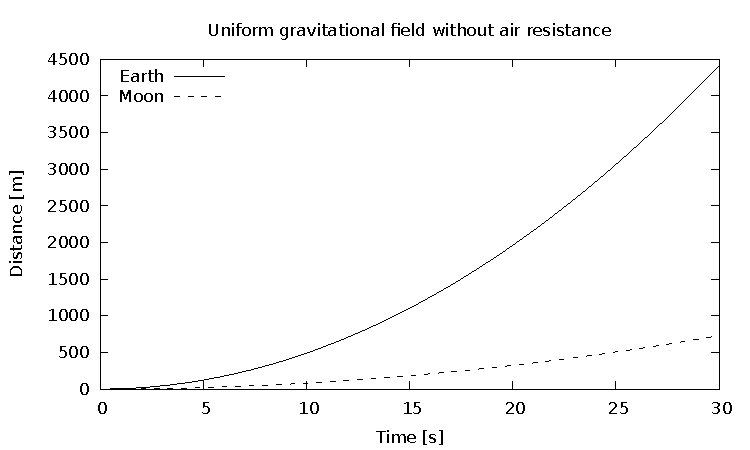
\includegraphics{gnuplot-bw}
% 	\caption{Černobílá varianta obrázku generovaného programem Gnuplot}\label{fig:gnuplot-bw}
% \end{figure}
% 
% \begin{figure}\centering
% 	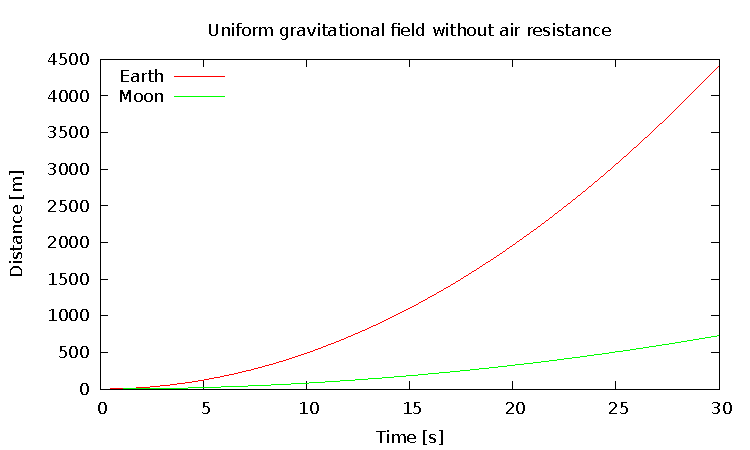
\includegraphics{gnuplot-col}
% 	\caption{Barevná varianta obrázku generovaného programem Gnuplot}\label{fig:gnuplot-col}
% \end{figure}
% 
% 
% \subsection{Tabulky}
% 
% Tabulky lze zadávat různě, např. v~prostředí \verb|tabular|, avšak pro jejich vkládání platí to samé, co pro obrázky -- použijte plovoucí prostředí, v~tomto případě \verb|table|. Například tabulka \ref{tab:matematika} byla vložena tímto způsobem.
% 
% \begin{table}\centering
% 	\caption[Příklad tabulky]{Zadávání matematiky}\label{tab:matematika}
% 	\begin{tabular}{|l|l|c|c|}\hline
% 		Typ		& Prostředí		& \LaTeX{}ovská zkratka	& \TeX{}ovská zkratka	\tabularnewline \hline \hline
% 		Text		& \verb|math|		& \verb|\(...\)|	& \verb|$...$|		\tabularnewline \hline
% 		Displayed	& \verb|displaymath|	& \verb|\[...\]|	& \verb|$$...$$|	\tabularnewline \hline
% 	\end{tabular}
% \end{table}
% 
% % % % % % % % % % % % % % % % % % % % % % % % % % % % 

\end{document}
